%%%%%%%%%%%%%%%%%%%%%%%%%%%%%%%%%%%%%%%%%%%%%%%%%%%%%%%%%%%%%%%%%%%%%%%%%%%%%%%%%%%%%%%%%%%%%
%%									Chapitre 2											%
%%%%%%%%%%%%%%%%%%%%%%%%%%%%%%%%%%%%%%%%%%%%%%%%%%%%%%%%%%%%%%%%%%%%%%%%%%%%%%%%%%%%%%%%%%%%%
\chapter{Stochastic Multi-Armed Bandits}\label{chap:mab}
	\citationChap{
	blabla
	}{}
	\minitoc
	\newpage

%%%%%%%%%%%%%%%%%%%%%%%%%%%%%%%%%%%%%%%%%%%%%%%%%%%%%%%%%%%%%%%%%%%%%%%%%%%%%%%%%%%%%%%%%%%%%

\section{The Multi-Armed Bandits Model}\label{sec:mab.model}

The problem of sequentially allocating resources to a defined set of actions (arms) based on successive \emph{partially observable} (see Definition~\ref{def:mab.mab} and Remark~\ref{remark:mab.partial} below) feedback refers to the MAB game in probability theory. The term \emph{bandit} is named, by analogy, after slot machines (or one-armed bandits) in a casino. A sequential decision making problem comes up then when facing with several slot machines (multi-armed bandits).

The study of MAB problems can date back to as early as 1933~\citep{thompson1933}, and was originally proposed to model sequential clinical trials. For example, researchers testing the efficacy of potential vaccines for a new coronavirus have to choose a vaccine (arm) from the following 4 options as shown in Fig.~\ref{fig:mab.covid} on each patient from an experimental group of $T$ person. For each patient $t\in[T]$, researchers receive a reward signal $r_t\in\{0,1\}$. $r_t=1$ indicates that the treatment is successful, otherwise the treatment is a failure. We thus assume that the efficacy of each vaccine follows some Bernoulli distribution that is unknown to the researchers.

\begin{figure}[ht]
    \centering
    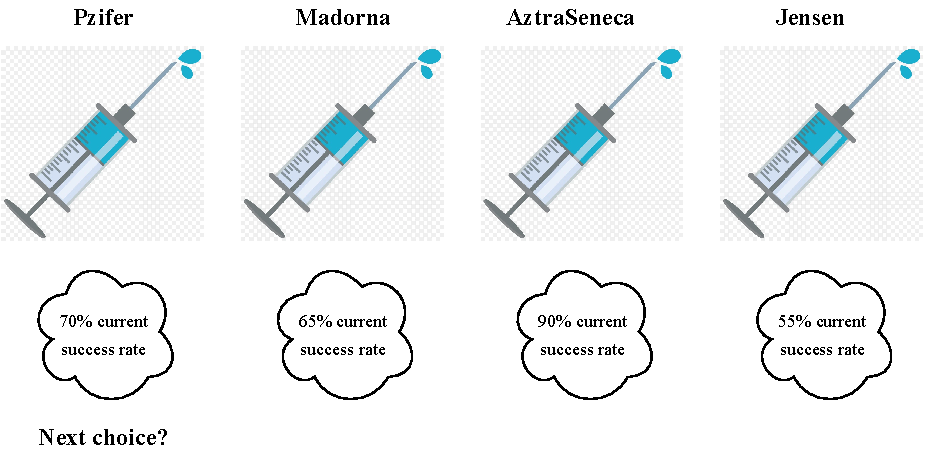
\includegraphics[width=\textwidth]{Chapter2/img/covid.pdf}
    \caption{An example of modelling clinical trials as a MAB problem.}
    \label{fig:mab.covid}
\end{figure}

As stated in Chapter~\ref{chap:intro}, a common learning objective for stochastic MAB is to maximize the total reward obtained given a sequence of observations. In the previous example, researchers need to decide which vaccine to employ for each patient depending on the previous success rates with the purpose of maximizing the total success rate $\sum_{t=1}^T r_t$ at the end.

However, due to the complex nature of medical treatment, it turns out that the MAB model is hardly applied in real clinical trials despite its primary purpose~\citep{reda2020drug}. Nevertheless, the model has been widely employed in many other applications recently, in particular online recommendation systems for example (see e.g.~\citealt{li2010contextual,zeng2016online}). Other application scenarios include...

In this section, we go a little beyond the intuition and provide the formal definition of the model. We also recall some fundamental results for the sake of self-containedness. Of course, we do not intend to write a survey of MAB, for which the content is far too rich for this thesis. Interested lecturers can refer to~\cite{bubeck2012bandits,lattimore2018bandits} or~\cite{slivkins2019bandits} for further readings and more general results.

\subsection{Problem Formulation}\label{sec:mab.model.formulation}

From a mathematical point of view, a MAB model is a collection of $K$ \emph{unknown} probability distributions $(\nu_k)_{1 \leq k \leq K}$. At each time step $t$, the learner chooses a distribution $\nu_{i_t}$ where $i_t\in[K]$ and receive a reward $r_t$ that is generated from $\nu_{i_t}$. We then recover the bandit learning cycle as shown in Fig.~\ref{fig:mab.mab}. We summarize such a sequential learning procedure in Definition~\ref{def:mab.mab}.

\begin{figure}[ht]
    \centering
    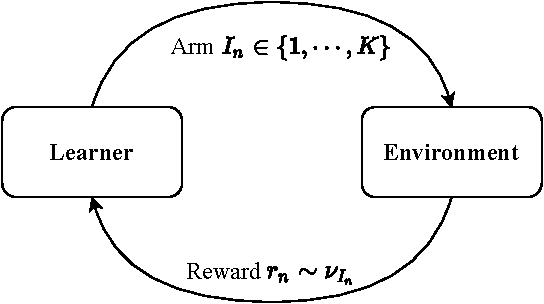
\includegraphics[width=0.5\textwidth]{Chapter2/img/mab_bis.pdf}
    \caption{A bandit learning cycle.}
    \label{fig:mab.mab}
\end{figure}

\begin{definition}[multi-armed bandit game]\label{def:mab.mab}
\begin{leftbar}[defnbar]
	We are given a set of $K$ arms $\{1,\cdots,K\}$ that follow $K$ unknown distributions $(\nu_k)_{1 \leq k \leq K}$, and a time horizon $T$. At each stage $t$, the bandit game consists of the following steps:
	\begin{itemize}
		\item a vector of rewards $(r_{1,t} \sim \nu_1, \cdots, r_{K,t} \sim \nu_K)$ is generated,
		\item the learner picks an arm $i_t \in \{1,\cdots,K\}$, and
		\item the learner observes the reward $r_t = r_{i_t, t}$.
	\end{itemize}
\end{leftbar}
\end{definition}

\begin{remark}\label{remark:mab.partial}
\begin{leftbar}[remarkbar]
	Rewards of unchosen arms at time $t$ are not revealed, this partial feedback setting is a special case of the online learning with experts setting.
\end{leftbar}
\end{remark}

In the rest of this manuscript, when $\nu_k$ are some common probability distributions, we can simply call our MAB model by the corresponding probability distribution name. For example, if the underlying reward distributions are Bernoulli (resp. Gaussian, exponential, Poisson, etc) distributions, then we can simply use Bernoulli bandits (resp. Gaussian bandits, exponential bandits, Poisson bandits, etc) to represent our bandit model. 

\subsection{Common assumptions on the rewards}\label{sec:mab.model.assumptions}

One important thing to take into consideration before starting any bandit game is to take care of the assumptions on the rewards. Intuitively, we shall have a minimum prior knowledge of the `shape' of the rewards. Obviously, the less the learner knows about that shape, the more difficult the problem is. In this thesis, several different assumptions on the reward distributions are considered depending on the problem settings. In the next, we offer a brief overview of commonly used assumptions in the literature.

\paragraph{Bounded rewards.}

The mostly considered assumption is whether the supports of the reward distributions are bounded, and if so, whether the bounds are known to the learner. In that latter case, we can assume without loss of generality that the rewards are supported on $[0,1]$. Indeed, if the rewards are contained in an arbitrary bounded interval $[a,b]$, then we can simply apply a normalization trick to recover the $[0,1]$ case.

The previous vaccine example of Fig.~\ref{fig:mab.covid} with Bernoulli bandits is a typical example of known bounded rewards. Bounded rewards are widely used in many MAB research work. It is also the case for instance in Chapter~\ref{chap:gpo} of this thesis.

\paragraph{One-dimensional exponential family.}

Unbounded reward distributions are obviously considered in the literature as well. An usual example of infinitely-supported reward distributions is Gaussian distribution. Therefore in the literature, we sometimes think of a more general parametric framework, namely the exponential family. The exponential family contains a large set of natural distributions as Bernoulli distributions and Gaussian distributions, hence covers a wide range of both bounded and unbounded rewards.

In practice, we often further consider a specific sub-family of distributions that is the \gls{one-dimensional exponential family} or \gls{single-parameter exponential family}. Typical distributions in the one-dimensional exponential family include beta distributions, Bernoulli distributions, Gaussian distributions with \emph{known} variance, etc. Formally, given a random variable $X$ whose probability distribution belongs to the single-parameter exponential family, then its \gls{probability density function} (or \gls{probability mass function} if $X$ is discrete), depending only on one single parameter $\theta$, can be written as
\begin{align}\label{eq:mab.exponential}
    p_{X}(x \mid \theta ) = b(x) \exp \left[\eta (\theta ) \cdot T(x) + A(\theta )\right]\,,
\end{align}
where $T(X)$ is the \gls{natural sufficient statistic} and $b,\eta,A$ are known functions. A more formal reminder of one-dimensional exponential family is given in Appendix~\ref{chap:maths}.

The MAB community is interested in exponential family not only because it covers a large family of most common distributions, but also because it holds some nice properties for statistical analysis. For example, exponential family has sufficient statistics that can summarize arbitrary amounts of \gls{iid} data with a finite number of samples, which is a great property in bandit analysis. Another important fact is that exponential family distributions have conjugate priors, which is extremely useful in Bayesian statistics. The latter one is for example used in Chapter~\ref{chap:t3c}.

\paragraph{Beyond...}

Other types of reward distributions are also studied in the literature. To list a few of them, we can think of sub-Gaussian distributions whose tails decay at least as fast as Gaussian distributions (see e.g.~\citealt{}), and also heavy-tailed distributions whose tails are not exponentially bounded (see e.g;~\citealt{yu2018heavy}). Those reward distributions also incite interesting theoretical questions as well as applications, but are out of the scope of this manuscript.

\subsection{Regret minimization}\label{sec:mab.model.regret}

Once we have imposed some assumptions on the reward distributions, the next step is to fix a learning goal and set an evaluation measure accordingly.

As previously stated that the classical learning objective of a MAB learner is to maximize the total return in the long run, hence trades-off between exploration and exploitation. To achieve that goal, the learner needs to design a clever (in a precise sense) way of pulling arms based on past observations, and we call this design an \emph{allocation strategy} or \emph{policy}. To evaluate a strategy under this reward maximization setting, one can use the metric often referred to as \emph{regret} defined in the next. 

Suppose that each unknown distribution $\nu_k$ is associated with a mean $\mu_k$, and that $\mu^{\star}$ is the mean of the optimal arm. One natural way to assess the quality of the given policy would be minimizing the total loss w.r.t the optimal arm during the whole process, which leads to the notion of \gls{cumulative regret} (sometimes simply called regret if there is no ambiguity).

\begin{definition}[cumulative regret]\label{def:mab.cumulative_regret}
\begin{leftbar}[defnbar]
	At the end of round $T$, a given policy which observes a sequence of rewards $(r_t)_{1 \leq t \leq T}$ suffers from a cumulative regret:
	\[
		\hat{R}_T \eqdef \max_{i=1\cdots K} \sum_{t=1}^T r_{i,t} - \sum_{t=1}^T r_t.
	\]
\end{leftbar}
\end{definition}

In general, both rewards and choices of the learner might be stochastic, it is thus often more convenient to consider a related \emph{pseudo-regret} that involves only the mean rewards $\mu_k$.

\begin{definition}[cumulative pseudo-regret]\label{def:mab.pseudo_regret}
\begin{leftbar}[defnbar]
	At the end of round $T$, a given policy which observes a sequence of rewards $(r_t)_{1 \leq t \leq T}$ suffers from a cumulative pseudo-regret:
	\[
		R_T \eqdef \mu^{\star}T - \sum_{t=1}^T \mu_{i_t}.
	\]
\end{leftbar}
\end{definition}

\begin{proposition}\label{prop:mab.pseudo_regret}
\begin{leftbar}[propositionbar]
	The expected value $\E[\hat{R}_T]$ of the cumulative regret and the expected value $\E[R_T]$ of the cumulative pseudo-regret are the same, where the expectation is taken with respect to both rewards and choices from the learner.
\end{leftbar}
\end{proposition}

\begin{proof}
	Let us define a function that relates each arm to its mean reward \func{f}{\{1,\cdots,K\}}{\R}{i_t}{\mu_{i_t}\,,} then by the tower rule, we have
    \[
	    \E[r_t] = \E[\E[r_t|i_t]] = \E[f(i_t)] = \mu_{i_t}\,.
    \]
\end{proof}

In practice, people are essentially interested in bounding: (a) the \emph{expected cumulative regret}, or (b) the \emph{cumulative regret with high probability}. One can notice that the two definitions of cumulative regret above are equivalent if their objective is to obtain an expected regret bound. People therefore often only focus on the pseudo-regret.

Clearly, minimizing the cumulative regret is equivalent to maximizing the total rewards, whence comes the name `regret minimization'. 

\subsection{Regret lower bound}

In Chapter~\ref{chap:intro} we have mentioned that regret minimization is not always the most appropriate learning objective under some circumstances, but we should rather study MAB from an optimization point of view. However, before we jump into details of MAB for optimization, let us briefly review some fundamental results of regret minimization as they may be relevant for understanding some of our motivations later.

The seminal work of~\cite{robbins1952}.

\section{Multi-Armed Bandits for Optimization}\label{sec:mab.optim}

The rest of this chapter is dedicated to MAB for optimization. We hereby aim to provide a formal presentation of different problem settings and related performance metrics. We put a specific focus of course on the settings to be investigated in this thesis.

\subsection{Best-arm identification for stochastic multi-armed bandits}

We begin by the original and simplest setting, namely BAI for stochastic MAB. Recall that in this case, we consider a finite-arm bandit model, which is a collection of $K$ probability distributions, called arms $\cX\eqdef\{x_1,\cdots,x_K\}$, parameterized by their means $\mu_1, \cdots, \mu_K$. When clear from the context, we can simply denote the arms by $\{1,2,\cdots,K\}$. We assume the (unknown) best arm is unique and we denote it by $I^\star \eqdef \argmax_i \mu_i$. 

A BAI strategy or algorithm can be characterized by a triple $(i_t, j_t, \tau)$ at each time step, hence consists of three components: 
\begin{itemize}
    \item The first is a \gls{sampling rule}, which selects an arm $i_t\in[K]$. Recall that in a MAB problem, a vector of rewards $(r_{t,1},\cdots,r_{t,K})$ is generated for all arms independently from past observations at each round, but only $r_t = r_{t,i_t}$ is revealed to the learner. Let $\cF_n$ be the $\sigma$-algebra generated by $(U_1,k_1,r_1,\cdots,U_t,i_t,r_t)$, then $i_t$ is $\cF_{t-1}$-measurable, i.e., it can only depend on the past $t-1$ observations, and some exogenous randomness, materialized into $U_{n-1} \sim \cU([0,1])$;
    \item The second component is a $\cF_{t}$-measurable \gls{decision rule} $j_t$, which returns a guess for the best arm;
    \item And thirdly, the \gls{stopping rule}~$\tau$, a stopping time with respect to $\left(\cF_{t}\right)_{t \in \mathbb{N}}$, decides when the exploration is over.
\end{itemize}

In general, there are two learning frameworks of BAI: (1) \gls{fixed-confidence setting}, first studied by~\citep{even-dar2003confidence} and (2) \gls{fixed-budget setting}, first proposed by~\citep{audibert2010budget}. The two frameworks differ in particular in the stopping rule that we precise in the next.

\paragraph{Fixed-confidence setting.}

In the fixed-confidence setting, the learner is given a confidence level/risk $\delta$ about the quality of the returned guess of the best arm. The goal is to reach a confidence of $1-\delta$ with as few samples as possible. Thus the fixed-confidence BAI can be summarized as follow.

\begin{definition}[fixed-confidence best-arm identification]\label{def:bai_confidence}
\begin{leftbar}[defnbar]
	We are given a set of $K$ arms $\{1,\cdots,K\}$ that follow $K$ unknown distributions $(\nu_k)_{1 \leq k \leq K}$, a confidence level $\delta$, and a stopping time $\tau$ w.r.t. the observations. At each time step $t$, the learning process consists of the following actions:
\begin{itemize}
	\item a vector of rewards $(r_{1,t} \sim \nu_1, \cdots, r_{K,t} \sim \nu_K)$ is generated,
	\item the learner picks an arm $i_t \in \{1,\cdots,K\}$ (according to the sampling rule),
	\item the learner observes the reward $r_t = r_{i_t, t}$,
	\item the learner stops if $\PP{j_{\tau}\neq i^{\star}} \leq \delta$, where $i^{\star}$ is the optimal arm, and
	\item the learner outputs a guess for the best arm $j_\tau \in \{1,\cdots,K\}$ (according to the decision rule) when they stop.
\end{itemize}
\end{leftbar}
\end{definition}

The goal is to obtain a small expected number of samples $\EEs{\bmu}{\tau}$, where $\bmu=(\mu_1,\mu_2,\cdots,\mu_K)$ is the underlying bandit model associated to the given set of $K$ arms. By the next of this chapter, we ignore the subscripts $\bmu$ for expectations and probabilities if there is no ambiguity. 

Most of the existing sampling rules rely on the confidence level $\delta$: Some of them rely on confidence intervals such as \LUCB~\citep{kalyanakrishnan2012lucb}, \UGapE~\citep{gabillon2012ugape}, \KLLUCB and \KLRacing~\citep{kaufmann2013kl}, and \LIL~\citep{jamieson2014lilucb}; others are elimination-based like \SE, \ME~\citep{even-dar2003confidence}, and \EGE~\citep{karnin2013sha}. The first algorithm that does not depend on $\delta$, \Track, is proposed by~\cite{garivier2016tracknstop}.

\paragraph{Fixed-budget setting}

In the fixed-budget setting, the learner tries to maximize the probability of returning the best (or $\epsilon$-best) arm with a fixed horizon $T$. Therefore, a policy in this case doen not require a stopping rule as the fixed-confidence setting does.

\begin{definition}[fixed-budget best-arm identification]
\begin{leftbar}[defnbar]
	We are given a set of $K$ arms $\{1,\cdots,K\}$ that follow $K$ unknown distributions $(\nu_k)_{1 \leq k \leq K}$, and a time horizon $T$. At each time step $t$, the learning process consists of the following actions:
\begin{itemize}
	\item a vector of rewards $(r_{1,t} \sim \nu_1, \cdots, r_{K,t} \sim \nu_K)$ is generated,
	\item the learner picks an arm $i_t \in \{1,\cdots,K\}$ (according to the sampling rule),
	\item the learner observes the reward $r_t = r_{i_t, t}$,
	\item the learner stops when $t=T$, and
	\item the learner outputs a guess for the best arm $j_T \in \{1,\cdots,K\}$ (according to the decision rule) when they stop.
\end{itemize}
\end{leftbar}
\end{definition}

The ultimate objective is thus to make the probability of $j_T$ not being the optimal arm, i.e. $\PP{j_T\neq i^{\star}}$, as small as possible. All of the existing fixed-budget sampling rules depend on the budget $T$. Just like the confidence setting, they either rely on lower and upper confidence bounds on the means of the arms like \UCBE~\citep{audibert2010budget}, and \UGapE~\citep{gabillon2012ugape}, or are based on arm eliminations such as \SR~\citep{audibert2010budget}, and \SHA~\citep{karnin2013sha}.

\paragraph{Anytime solutions}

The fact that the two previous settings provide a sampling rule that depends either on a confidence parameter $\delta$ or a budget parameter $n$ is not desirable in some real applications. To address this problem, \cite{jun2016atlucb} propose to use a \emph{doubling trick} upon fixed-budget algorithms like \SR and \SHA, or use a time-varying confidence parameter when dealing with the fixed-confidence setting. This allows us to stop the learning process \emph{anytime} we want, meaning that we want the probability of $i^{\star}$ not being recommended to be decreasing as fast as possible. \cite{russo2016ttts} provides an interesting alternative that evaluates sampling rules in a Bayesian perspective. In this note, our main interest remains on how to develop universal anytime BAI algorithms.

Now that we know that a BAI algorithm is composed of a sampling rule and a decision rule, sometimes coupled with a stopping rule. For the rest of this chapter, we first introduce several common recommendation strategies before entering into details of different fixed-budget or fixed-confidence sampling strategies. 

\paragraph{decision rules}

There exist several natural and simple decision rules that can be applied to most of the existing BAI algorithms, namely \emph{empirical best arm} (\EBA), \emph{most played arm} (\MPA) and \emph{empirical distribution of plays} (\EDP)~\citep{bubeck2009pure}.

\begin{remark}
The present strategies are obviously not the only options for recommendations, we introduce later in this chapter different strategies that are specific to some sampling rules.
\end{remark}

\paragraph{Sampling rules}

In a fixed-confidence BAI problem, a sampling rule is always accompanied by a stopping rule that decides when to stop the algorithm given a confidence level $\delta$. This stopping rule is characterized by a $\delta$-dependent stopping time $\tau_{\delta}$. As we stated in the introduction of this chapter, our goal is to minimize its expectation $\EEs{\bmu}{\tau_{\delta}}$. By Definition~\ref{bai_confidence}, it is clear to see that we are searching for a \emph{probably approximately correct} (PAC) algorithm~\citep{valiant1984pac} in a fixed-confidence BAI frame.

\begin{definition}[$\delta$-PAC strategy]
An algorithm (sampling rule) is called $\delta$-PAC if for any bandit model, we have
\[
	\PP{\tau_\delta < \infty} = 1 \text{ and } \PP{j_{\tau_\delta}\neq i^{\star}} \leq \delta.
\]
\end{definition}

\subsection{Best-arm identification for linear bandits}

\subsection{Other variants of best-arm identification}

\subsection{$\cX$-armed bandits}

\section{Performance Measure}\label{sec:mab.performance}

\subsection{Optimization error}

\subsection{Sample complexity}

\subsection{Simple regret}

\begin{definition}[simple regret]\label{def:stoch_mab.simple_regret}
\begin{leftbar}[defnbar]
	At the end of round $T$, a given policy which observes a sequence of rewards $(r_t)_{1 \leq t \leq T}$ and a recommendation $j_T$ suffers from a simple regret:
	\[
		S_T \eqdef \mu^{\star} - \mu_{j_T}\,.
	\]
\end{leftbar}
\end{definition}